\chapter{Abschätzen von Parametern}
\label{chap:estimation}

\section{Bayessche Datananalyse}
\label{chap:estimation:sec:bayes}

Die Bayessche Analyse präsentiert ein vollkommen anderes Verständnis von Wahrscheinlichkeiten als der frequentistische Ansatz, der in Kapitel \ref{chap:fehler:sec:frequentistisch} behandelt wurde. In diesem Ansatz wird die Unsicherheit als eine subjektive Unsicherheit anstelle einer objektive Unsicherheit des Experiments interpretiert. Während der frequentistische Ansatz eine hohe Anzahl an Wiederholungen eines Experimentes erfordert, um Wahrscheinlichkeiten zu berechnen und aufgrund derer Aussagen über die Zukunft zu treffen, bilden im Bayesschen Ansatz subjektive Erfahrungen die Grundlage dafür. Im Fokus der Bayesschen Analyse stehen daher bedingte Wahrscheinlichkeiten und der Satz von Bayes (siehe Gleichung \ref{eq:bayes}) nimmt eine zentrale Stellung ein. Im Folgenden definieren wir
\begingroup
\setlength{\tabcolsep}{10pt} % Default value: 6pt
\renewcommand{\arraystretch}{1.5} % Default value: 1
\begin{table}[H]
\begin{tabular}{l|l}
Die gemessenen Daten des Experiments                                        & $A \rightarrow D$                                 \\
\multirow{2}{*}{\shortstack[l]{Ein endlicher Satz von Ergebnissen, die wir\\
mithilfe der Daten unterscheiden möchten}}                                & \multirow{2}{*}{$B \rightarrow B_1, ..., B_n$} \\
   &       \\
Unser gesamtes zusätzliches Wissen (wird oft vernachlässigt)            & I 
\end{tabular}
\end{table}
\endgroup
und schreiben den Satz von Bayes damit als
\begin{align}
P ( B_i | D, I ) = \frac{ P ( D | B_i, I) P ( B_i | I )}{ P ( D | I ) }\,
\label{eq:bayesrewritten}
\end{align}
oder vereinfacht zu
\begin{align}
P ( B_i | D ) = \frac{ P ( D | B_i) P ( B_i )}{ P ( D ) }\,.
\label{eq:bayesrewrittensimple}
\end{align}
Wenn $D$ impliziert, dass eines der $B_i$ eintritt, gilt weiterhin
\begin{align}
P ( D ) = \sum_k P ( D | B_k ) P ( B_k )\,.
\end{align}

In Gleichung \ref{eq:bayesrewrittensimple} ist $P(B_i)$ die \textit{a-priori} Wahrscheinlichkeit für das Eintreten eines Ergebnisses $B_i$ die auf dem ursprünglichen Wissen \textit{vor} der Durchführung eines Experiments basiert. Es werden nun eine Reihe von Daten $D$ gemessen und die konditionellen Wahrscheinlichkeiten $ P(D|B_i)$ für deren Auftreten in Abhängigkeit des Vorliegens eines bestimmten Ergebnisses $B_i$ berechnet. Die Kenntnis der $P(B_i)$ und $ P(D|B_i)$ ermöglicht es nun, sogenannte \textit{a-posteriori} Wahrscheinlichkeiten $ P(B_i|D)$ zu bestimmen, mit denen ein Ergebnis $B_i$ basierend auf der Grundlage des Datensatzes $D$ auftritt. Es wird also eine subjektive Erfahrung, die Kenntnis des Datensatzes $D$, zur Berechnung der Wahrscheinlichkeiten verwendet.


\begin{center}
\begin{tcolorbox}[enhanced,width=6in,drop fuzzy shadow southwest,
colframe=blue!50!black,colback=blue!01]
\textbf{Beispiel 1}: Die Infektionskrankheit \\
 Nehmen wir an, es gibt eine Infektionskrankheit mit einer Inzidenzrate von 100. Das bedeutet, dass 100 von 100000 Menschen, also 0.1 \%, infiziert sind.  Die \textit{a-priori} Wahrscheinlichkeiten dafür, ob eine Person infiziert ($B_I$) oder gesund ($B_G$) ist, sind somit
 \begin{align}
 P(B_I) = 0.001 \label{eq:proability-example}
 \end{align}
  \begin{align}
 P(B_G) = 0.999 \label{eq:proability-example2}
 \end{align}
 Eine Person lässt sich nun testen und der Test ist positiv. Wie hoch ist die Wahrscheinlichkeit, dass die Person tatsächlich infiziert ist, wenn der Test in 99\% der Fälle das korrekte Ergebnis liefert?  \\

 Um diese Frage zu beantworten, berechnen wir zuerst die bedingten Wahrscheinlichkeiten
 \begin{align}
P(D|B_I) = 0.99
 \end{align}
  \begin{align}
P(D|B_G) = 0.01
 \end{align}
und verwenden dann den Satz von Bayes. Dieser liefert
\begin{align}
P(B_I|D) = \frac{P(D|B_I)P(B_I)}{P(D|B_I)P(B_I) + P(D|B_G)P(B_G)} = 0.1,
\end{align}
die Wahrscheinlichkeit, dass die Person tatäschlich infiziert ist, liegt somit \glqq nur\grqq  bei 10\%. \\

Wenn sich die Person nun ein weiteres Mal testen lässt und der Test erneut positiv ist, verwenden wir nun die aus dem ersten Testergebnis resultierenden Wahrscheinlichkeiten $P(B_I) = 0.1$ und $P(B_G) = 0.9$ als neue \textit{a-priori} Wahrscheinlichkeiten und verwenden auf dieser Grundlage erneut den Satz von Bayes. Nach der zweiten positiven Testrunde ergibt diese Berechnung, dass die Person zu 92\% infiziert ist. 
\end{tcolorbox}
\end{center}


\begin{center}
\begin{tcolorbox}[enhanced,width=6in, drop fuzzy shadow southwest,
colframe=blue!50!black,colback=blue!01]
\textbf{Beispiel 2}: Das Ziegenproblem \\

Hinter lediglich einem von drei Toren befindet sich eine Ziege. Ziel eines Spiels ist es nun, zu erraten, hinter welchem der Tore sich die Ziege befindet. Der Kandidat des Spiels wird dazu aufgefordert, sich für ein Tor $i=$1, 2 oder 3 zu entscheiden. Anschliessend öffnet der Moderator des Spiels eins der beiden Tore, für das sich der Spieler nicht entschieden hat und hinter dem sich die Ziege \textit{nicht} befindet. Der Kandidat erhält nun die Möglichkeit, entweder auf seiner ursprünglichen Wahl zu bestehen oder seine Meinung nochmals zu ändern. Mit welcher Entscheidung gewinnt er das Spiel mit höherer Wahrscheinlichkeit? \\

Diese Frage lässt sich mithilfe des Satz von Bayes beantworten. Die Wahrscheinlichkeiten $P(B_i)$, das sich die Ziege hinter dem Tor $i$ befindet ist für alle Tore identisch und gleich $\frac{1}{3}$. Nehmen wir nun ein konkretes Szenario an, indem sich der Spieler für ein Tor $k=1$ entscheidet und der Moderator anschliessend das Tor $j=3$ öffnet. Die bedingten Wahrscheinlichkeiten $P(D|B_i)$, dass dieses Ergebnis $D$ eintritt, wenn sich die Ziege hinter einem Tor $i$ befindet, sind somit
\begin{align}
P(D|B_1)\cdot P(B_1) = \frac{1}{2} \cdot \frac{1}{3} = \frac{1}{6} 
\end{align}
\begin{align}
P(D|B_2)\cdot P(B_2) = 1 \cdot \frac{1}{3} = \frac{1}{3}
\end{align}
\begin{align}
P(D|B_3)\cdot P(B_3) = 0 \cdot \frac{1}{3} = 0
\end{align}
Mithilfe des Satzes von Bayes können wir nun die Wahrscheinlichkeiten $P(B_1|D)$ und $P(B_2|D)$ berechnen:
\begin{align}
\begin{split}
P(B_1|D) = \frac{P(D|B_1)P(B_1)}{P(D|B_1)P(B_1) + P(D|B_2)P(B_2) + P(D|B_3)P(B_3)} = \frac{1}{3}
\end{split}
\end{align}

\begin{align}
\begin{split}
P(B_2|D) = \frac{P(D|B_2)P(B_2)}{P(D|B_1)P(B_1) + P(D|B_2)P(B_2) + P(D|B_3)P(B_3)} = \frac{2}{3}
\end{split}
\end{align}
Der Spieler erhöht (verdoppelt) somit seine Gewinnchancen, wenn er seine Wahl nochmals ändert.
\end{tcolorbox}
\end{center}





\section{Likelihood Funktion und Maximum Likelihood}\label{sec:likelihood}

\begin{center}
\begin{tcolorbox}[enhanced,width=6in,center upper,
    fontupper=\large,drop fuzzy shadow southwest,
    colframe=blue!50!black,colback=blue!10]
    {Zur Likelihood Funktion und Maximum Likelihood ist ein Jupyter-Notebook verfügbar. Siehe \gitresource{Likelihood Function.ipynb} }
\end{tcolorbox}
\end{center}

\subsection{Likelihood-Funktion}
\label{subsec:vl8}


Wir haben gesehen, dass eine einzelne Messung äquivalent ist zu einer Ziehung einer Zufallszahl aus einer Wahrscheinlichkeitsverteilung. Die Wahrscheinlichkeitsverteilung einer Zufallsvariable \gls{gl:zeta} sei:
\begin{align}
f(\zeta, a_0, a_1, ..., a_m) = f (\zeta, \boldsymbol{a})\,.
\label{eq:vl8-1}
\end{align}

Hierbei ist $\boldsymbol{a}$ ein Vektor der die Wahrscheinlichkeitsverteilung parametrisiert, wie z. B. in Gl. (\ref{eq:proability-example}) und (\ref{eq:proability-example2}). F\"ur mehrere Variablen schreiben wir: 
\begin{align}
f(\zeta_0, \zeta_1, ..., \zeta_n, a_0, a_1, ..., a_m) = f (\boldsymbol{\zeta}, \boldsymbol{a}).\,
\label{eq:vl8-2}
\end{align}

In einem Experiment sind die Werte der $a_i$ unbekannt, aber wir kennen (aus der Messung) einige $\zeta_i$, zum Beispiel messen wir die Werte $\zeta_i = x_i$. Also k\"onnen wir schreiben:
\begin{align}
f(x_0, x_1, ..., x_n, \boldsymbol{a}) = f(\boldsymbol{x, a}) \overset{\text{def}}{=} L (\boldsymbol{x,a})\,.
\label{eq:vl8-3}
\end{align}

\begin{center}
\begin{tcolorbox}[enhanced,width=6in,drop fuzzy shadow southwest,
    colframe=red!50!black,colback=red!05]
   Hierbei ist $L$ die Likelihood-Funktion. In der Likelihood-Funktion sind die $x_i$ bekannt und die $a_i$ sind die Variablen.
\end{tcolorbox}
\end{center}


\textit{Beispiel: Wir messen zwei unabh\"angige Datenpunkte $x_1$ und $x_2$ aus einer Gaussverteilung:}
\begin{align}
f(\zeta, a_0, a_1) = \frac{1}{ \sqrt{ 2 \pi a_1 } } \exp \left( - \frac{1}{2} \frac{ (\zeta - a_0)^2 }{ a_1 } \right)\,.
\label{eq:vl8-4}
\end{align}

\textit{Die Parameter $a_0$ (der Erwartungswert) und $a_1$ (die Varianz) sind unbekannt. Da die Messungen unabh\"angig sind, ist die gemeinsame Wahrscheinlichkeitsverteilung das Produkt der Einzelwahrscheinlichkeiten:}
\begin{align}
f(x_1, x_2, a_0, a_1) &= f(x_1, a_0, a_1)f(x_2, a_0, a_1) = \frac{1}{ 2 \pi a_1 } \exp \left( - \frac{1}{2} \frac{ \sum_{i=1}^2 (x_i - a_0)^2 }{ a_1 } \right)\,. \\
L(x_1, x_2, a_0, a_1) &= f(x_1, x_2, a_0, a_1)
\label{eq:vl8-5}
\end{align}

In diesem Beispiel sieht die Likelihood-Funktion der Wahrscheinlichkeitsverteilung sehr \"ahnlich. Aber Vorsicht:

\begin{center}
\begin{tcolorbox}[enhanced,width=6in,drop fuzzy shadow southwest,
    colframe=red!50!black,colback=red!05]
   Die Likelihood-Funktion ist \textbf{keine} Wahrscheinlichkeitsverteilung. Die Likelihood-Funktion ist eine Plausibilitätsfunktion.
\end{tcolorbox}
\end{center}

Insbesondere ist sie nicht normiert.\\[0.3cm]
\textit{Beispiel: Wir haben einen Satz von Widerst\"anden mit einer unbekannten Toleranz, wie in Abb. \ref{fig:likelihood}, links als Histogramm gezeigt.
Wir nehmen an, dass die Widerstandswerte normalverteilt sind. F\"ur $n$ Datenpunkte $\boldsymbol{x} = (x_1, x_2, ..., x_n)$ gilt dann:}
\begin{align}
L(\boldsymbol{x}, a_0, a_1) =  \prod_{i = 1}^n f(x_i, a_0, a_1) = \left( \frac{1}{ 2 \pi a_1 } \right)^\frac{n}{2} \exp \left( - \frac{1}{2} \frac{ \sum_{i=1}^n (x_i - a_0)^2 }{ a_1 } \right)\,.
\label{eq:vl8-6}
\end{align}

\begin{figure}[tbp]
    \centering
        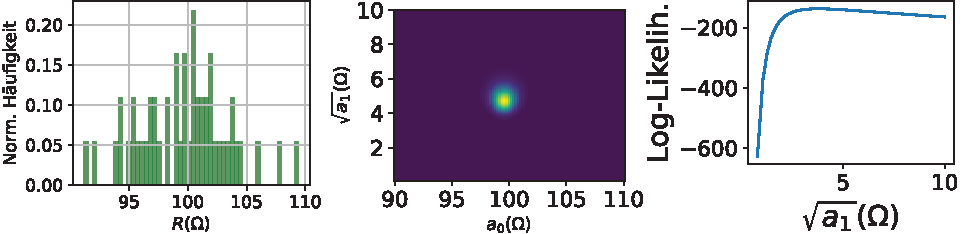
\includegraphics[width=0.8\textwidth]{Figures/likelihood_funktion.pdf}
        \caption{Beispiel zur Likelihood Funktion \textbf{Links:} Histogramm von "gemessenen" Widerstandswerten. \textbf{Mitte:} Likelihood Funktion für verschiedene Parameter $a_{0,1}$ der zugrunde liegendenden Normalverteilung. \textbf{Rechts:} Log-Likelihood Funktion der gleichen Daten. }
        \label{fig:likelihood}
\end{figure} 

\textit{Wir berechnen die Likelihood-Funktion f\"ur ``alle'' Werte von $a_0$ und $a_1$. 
Das Ergebnis ist in Abb. \ref{fig:likelihood}, Mitte zu sehen. 
Wir finden die maximale Likelihood f\"ur eine Verteilung bei $\hat{a}_0 = 100\,\Omega$ und $\sqrt{\hat{a}_1} = 5\,\Omega$.\\
In diesem Fall, weil die Daten normalverteilt sind, h\"atten wir auch die Ausdr\"ucke f\"ur die Absch\"atzung von Erwartungswert und Standardabweichung benutzen k\"onnen. Aber die Analyse der Likelihood-Funktion funktioniert auch bei beliebigen anderen Verteilungen.}


\subsection{Maximum Likelihood}
\label{subsec:vl8-2}

Der genaue Wert der Likelihood-Funktion ist nicht besonders aussagekr\"aftig. Weil sie nicht normiert sein muss, gibt sie uns keine Wahrscheinlichkeit bzw. Wahrscheinlichkeitsdichte. Aber die Likelihood-Funktion beinhaltet Information \"uber die Parameter $\boldsymbol{a}$ der Wahrscheinlichkeitsverteilung. Sie gibt uns eine Plausibilität für die Werte der Parameter $\boldsymbol{a}$. Daher sind Werte von $\boldsymbol{a}$, die eine grosse Likelihood haben, zu bevorzugen.\\[0.3cm]
Wir k\"onnen Likelihoods \"uber ihr Verh\"altnis vergleichen:
\begin{align}
LR = \frac{L(\boldsymbol{x,a})}{L(\boldsymbol{x,b})}\,.
\label{eq:vl8-7}
\end{align}

Dies ist das Verh\"altnis der ``Plausibilitäten'', dass die Parameter $\boldsymbol{a}$ und $\boldsymbol{b}$ die gemessenen Daten erkl\"aren. Insbesondere wollen wir die Werte f\"ur $\boldsymbol{a}$ finden, die die Likelihood-Funktion maximieren.

\begin{center}
\begin{tcolorbox}[enhanced,width=6in,drop fuzzy shadow southwest,
    colframe=red!50!black,colback=red!05]
   Dies ist das sogenannte \textbf{Maximum Likelihood}-Prinzip. 
\end{tcolorbox}
\end{center}


Wir beginnen wieder mit gaussverteilten Daten $\boldsymbol{x} = (x_1, x_2, ..., x_n)$. Die zugrundeliegende Likelihood-Funktion ist:
\begin{align}
f(\zeta, a_0, a_1) = \frac{1}{ \sqrt{2 \pi a_1} } \exp \left( - \frac{1}{2} \frac{ (\zeta - a_0)^2 }{ a_1 } \right)\,.
\label{eq:vl8-8}
\end{align}

Die Parameter $a_0$ (der Erwartungswert) und $a_1$ (die Varianz) sind wieder unbekannt und wir wollen diese Werte absch\"atzen. Die kombinierte Likelihood-Funktion ist dann das Produkt der einzelnen Likelihood-Funktionen:
\begin{align}
L(\boldsymbol{x}, a_0, a_1) =  \left( \frac{1}{ 2 \pi a_1 } \right)^\frac{n}{2} \exp \left( - \frac{1}{2} \frac{ \sum_{i=1}^n (x_i - a_0)^2 }{ a_1 } \right)\,.
\label{eq:vl8-9}
\end{align}

Wir sind ausschliesslich an den Werten von $a_0$, $a_1$ interessiert die diese Funktionen maximieren, aber nicht am Wert des Maximums. Wir k\"onnen also den Logarithmus nehmen (Damit l\"asst sich leichter rechnen.):
\begin{align}
\gls{gl:logl}(x, a_0, a_1) = - \frac{n}{2} \ln{ ( 2 \pi a_1 ) } - \frac{1}{2} \frac{ \sum_{i=1}^n (x_i - a_0)^2 }{ a_1 }\,.
\label{eq:vl8-10}
\end{align}

\begin{center}
\begin{tcolorbox}[enhanced,width=6in,drop fuzzy shadow southwest,
    colframe=red!50!black,colback=red!05]
   Dies ist die sogenannte \textbf{Log-Likelihood-Funktion. }
\end{tcolorbox}
\end{center}

In Abb. \ref{fig:likelihood}, rechts, ist die Log-Likelihood Funktion für das Beispiel im vorigen Abschnitt zu sehen. \\

Wir wollen also die Log-Likelihood-Funktion (\cref{eq:vl8-10}) maximieren. Also berechnen wir die Ableitung von $l$ nach $a_0$ und $a_1$ an dem Stellen $\hat{a}_0$ und $\hat{a}_1$ und setzen diese gleich Null, sodass $\hat{a}_0$ und $\hat{a}_1$ dann die Werte sind, die $l$ maximieren:
\begin{align}
\begin{split}
\frac{ \partial l }{ \partial a_0 } &= \frac{ \partial }{ \partial a_0 } \bigg|_{\hat{a}_0, \hat{a}_1} - \frac{n}{2} \ln{ ( 2 \pi a_1 ) } - \frac{1}{2} \frac{ \sum_{i=1}^n (x_i - a_0)^2 }{ a_1 } = 0\,,\\
\rightarrow 0 &= \frac{1}{ \hat{a}_1} \sum_{i = 1}^n (x_i - \hat{a}_0)\,,\\
&=  \frac{1}{ \hat{a}_1} \left( \sum_{i = 1}^n x_i - n \hat{a}_0 \right)\\
\text{Der Erwartungswert:}\quad \quad \rightarrow \hat{a}_0 &= \frac{1}{n} \sum_{i = 1}^n x_i\\
\label{eq:vl8-11}
\end{split}
\end{align}
und:
\begin{align}
\begin{split}
\frac{ \partial l }{ \partial a_1 } &= \frac{ \partial }{ \partial a_1 } \bigg|_{\hat{a}_0, \hat{a}_1} - \frac{n}{2} \ln{ ( 2 \pi a_1 ) } - \frac{1}{2} \frac{ \sum_{i=1}^n (x_i - a_0)^2 }{ a_1 } = 0\,,\\
\rightarrow 0 &= - \frac{n}{2}\frac{1}{ \hat{a}_1 } + \frac{1}{ 2 \hat{a}_1^2 }\sum_{i = 1}^n (x_i - \hat{a}_0)^2\,,\\
\text{Die Varianz:}\quad \quad \quad \quad \quad \enspace
\rightarrow \hat{a}_1 &= \frac{1}{n} \sum_{i = 1}^n (x_i - \hat{a}_0)^2\,.
\label{eq:vl8-12}
\end{split}
\end{align}

Bemerkung: Der Wert der Varianz hat einen Bias im Vergleich zu dem Wert f\"ur die empirische Varianz.


\subsection{Der gewichtete Mittelwert}
\label{subsec:vl8-3}

Wir betrachten nun ein h\"aufiges Szenario. Wir messen mit einer uns bekannten und charakterisierten Messapparatur. Das heisst die Messunsicherheit (die Standardabweichung) $\sigma_i$ jeder Messung ist bekannt. Wir messen den Datensatz $\boldsymbol{x} = (x_1, x_2, ..., x_n)$ und wollen den Mittelwert bestimmen.\\
Die zugrundeliegende Likelihood-Funktion jeder Messung ist:
\begin{align}
f_i(\zeta_i, \sigma_i, a) = \frac{1}{ \sqrt{2 \pi } \sigma_i} \exp \left( - \frac{1}{2} \frac{ (\zeta - a)^2 }{ \sigma_i^2 } \right)\,.
\label{eq:vl8-13}
\end{align}

Damit is die Likelihood-Funktion:
\begin{align}
L(\boldsymbol{x,\sigma}, a) = \prod_{i=1}^n \frac{1}{ \sqrt{2 \pi } \sigma_i} \exp \left( - \frac{1}{2} \frac{ (x_i - a)^2 }{ \sigma_i^2 } \right)
\label{eq:vl8-14}
\end{align}

und die Log-Likelihood-Funktion:
\begin{align}
l(\boldsymbol{x,\sigma}, a) = \sum_{i=1}^n \ln \left( \frac{1}{ \sqrt{2 \pi } \sigma_i} \right) - \frac{1}{2} \sum_{i=1}^n \frac{ (x_i - a)^2 }{ \sigma_i^2 }\,.
\label{eq:vl8-15}
\end{align}

Wir bestimmen das Maximum:
\begin{align}
\begin{split}
\frac{ \partial l }{ \partial a } \bigg|_{\hat{a}} &= \frac{ \partial }{ \partial a } \bigg|_{\hat{a}} \left( - \frac{1}{2} \sum_{i=1}^n \frac{ (x_i - a)^2 }{ \sigma_i^2 } \right) = 0\,,\\
\rightarrow \sum_{i=1}^n \frac{ x_i - \hat{a} }{ \sigma_i^2 } &=  \sum_{i=1}^n \frac{ x_i }{ \sigma_i^2 } - \hat{a} \sum_{i=1}^n \frac{ 1 }{ \sigma_i^2 }\,,\\
\rightarrow \hat{a} &= \frac{ \sum_{i=1}^n \frac{ x_i }{ \sigma_i^2 } }{ \sum_{i=1}^n \frac{ 1 }{ \sigma_i^2 } } =\frac{ \sum_{i=1}^n w_i x_i }{ \sum_{i=1}^n w_i \,}.
\label{eq:vl8-16}
\end{split}
\end{align}

Hier definieren wir das Gewicht der einzelnen Messwerte als $w_i = \frac{1}{\sigma_i^2}$. 
Letzteres ist der \textbf{gewichtete Mittelwert}. Das heisst die einzelnen Werte $x_i$ tragen zum Wert des Mittelwertes mehr bei, wenn sie eine kleinere Unsicherheit haben. Werte mit grosser Unsicherheit haben dementsprechend einen kleineren Beitrag zum Mittelwert.



\chapter{Fitten von Parametern}
 
\section{Lineares Fitten von Polynomen}
\begin{center}
\begin{tcolorbox}[enhanced,width=6in,center upper,
    fontupper=\large,drop fuzzy shadow southwest,
    colframe=blue!50!black,colback=blue!10]
    {Zum linearen Fitten ist ein Jupyter-Notebook verfügbar. Siehe \gitresource{linear\_fitting.ipynb} }
\end{tcolorbox}
\end{center}

\subsection{Die Methode der kleinsten Quadrate}
\label{subsec:vl8-4}

Bisher haben wir die Likelihood-Funktion maximiert, um Parameter zu bestimmen, die die Wahrscheinlichkeitsverteilung (PDF) eines Datensatzes beschreiben. Insbesondere die Log-Likelihood-Funktion ist einfach zu maximieren wenn die PDF eine Gaussverteilung ist:
\begin{align}
\frac{ \partial l }{ \partial a } \bigg|_{\hat{a}} &= \frac{ \partial }{ \partial a } \bigg|_{\hat{a}} \left( - \frac{1}{2} \sum_{i=1}^n \frac{ (x_i - a)^2 }{ \sigma_i^2 } \right) = 0\,.
\label{eq:vl8-17}
\end{align}

In diesem Fall ist die Maximierung der Log-Likelihood-Funktion \"aquivalent zur Minimierung der Summe der  Abstandsquadrate der einzelnen Messpunkte zum Erwartungswert (also dem Modell). Dies ist die Methode der kleinsten Quadrate.
Wir definieren die Summe der Abstandsquadrate $S = \sum_{i=1}^n \frac{ (x_i - a)^2 }{ \sigma_i^2 }$ und damit schreiben wir:
\begin{align}
\frac{ \partial S }{ \partial a } \bigg|_{\hat{a}} &= \frac{ \partial }{ \partial a } \bigg|_{\hat{a}} \sum_{i=1}^n \frac{ (x_i - a)^2 }{ \sigma_i^2 } = 0\,.
\label{eq:vl8-18}
\end{align}

Bemerkung: Wenn die $\sigma_i$ bekannt sind, dann ist dies \"aquivalent zur Minimierung von $\chi^2$ und damit ist $S = \chi^2$. Das ist jedoch oft nicht der Fall, wir bleiben also zun\"achst bei $S$.


\subsection{Lineares Fitten von Polynomen}
\label{subsec:vl8-5}

\begin{figure}[tbp]
    \centering
        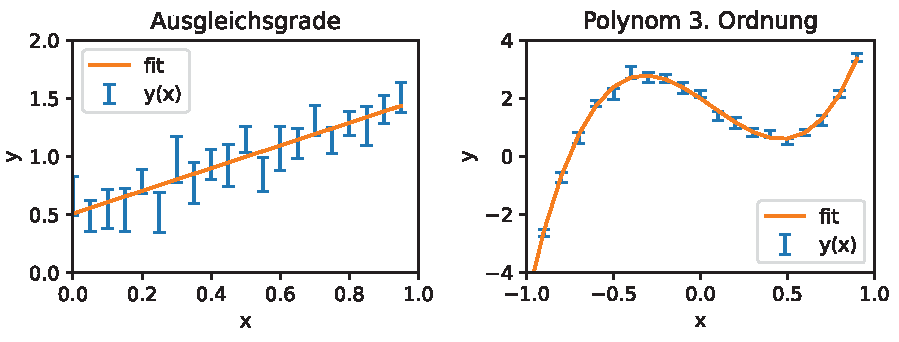
\includegraphics[width=0.8\textwidth]{Figures/linear_fitting_image.pdf}
        \caption{Beispiel zum linearen Fitten. \textbf{Links:} Linearer Fit einer Ausgleichsgerade zu fehlerbehafteten Daten. \textbf{Rechts:} Linearer Fit eines Polynoms dritten Grades an fehlerbehafteten Daten. }
        \label{fig:linearFit}
\end{figure} 

\subsubsection{Fitten einer Ausgleichsgeraden}
\label{subsubsec:vl8}

Wir haben die Werte $y_1, y_2, ..., y_n$ als Funktion der Kontrollparameter $x_1, x_2, ..., x_n$ gemessen. Die $x_i$ haben keine Unsicherheit, w\"ahrend die Unsicherheiten der $y_i$ durch $\sigma_i$ gegeben sind. Das bedeutet, dass die Wahrscheinlichkeit, dass der Wert $y$ gemessen wird gegeben ist durch:
\begin{align}
f(y) \sim \exp \left( - \frac{ (y - \mu)^2 }{ 2 \sigma^2 } \right)\,,
\label{eq:vl8-19}
\end{align}

wobei beide Werte $y$ und $\sigma$ von $x$ abh\"angen. Wir nehmen an, dass $\mu = a_0 + a_1 x$, also dass die Erwartungswerte von $y$ linear von $x$ abh\"angen, wie in Abb. \ref{fig:linearFit}, links zu sehen ist. Wir wollen die Werte von $a_0$ und $a_1$ finden, die die Daten am besten wiedergeben. Das heisst:
\begin{align}
f(y) \sim \exp \left( - \frac{ (y - a_0 - a_1 x_i)^2 }{ 2 \sigma_i^2 } \right)
\label{eq:vl8-20}
\end{align}

ist die Wahrscheinlichkeitsverteilung der $y_i$. Dann ist die Likelihood-Funktion f\"ur den $i-$ten Datenpunkt:
\begin{align}
L(x_i, y_i, \sigma_i, a_0, a_1) \sim \exp \left( - \frac{ (y_i - a_0 - a_1 x_i)^2 }{ 2 \sigma_i^2 } \right)
\label{eq:vl8-21}
\end{align}

und die kombinierte Log-Likelihood-Funktion für alle Datenpunkte:
\begin{align}
l(\boldsymbol{x, y, \sigma}, a_0, a_1) = - \frac{1}{2} \sum_{i=1}^n \frac{ (y_i - a_0 - a_1 x_i)^2 }{ \sigma_i^2 } + C
\label{eq:vl8-22}
\end{align}

mit einer Konstanten $C$. Wir benutzen wieder die Gewichte $w_i= \frac{1}{\sigma_i^2}$ und damit ist:
\begin{align}
l(\boldsymbol{x, y, w}, a_0, a_1) = - \frac{1}{2} \sum_{i=1}^n w_i (y_i - a_0 - a_1 x_i)^2 + C\,.
\label{eq:vl8-23}
\end{align}

Wir k\"onnen die besten Absch\"atzungen f\"ur $a_0$ und $a_1$ finden, indem wir die partiellen Ableitungen von $l$ nach $a_0$ und $a_1$ gleich Null setzen. Da die Unsicherheiten einer Normalverteilung zugrunde liegen, k\"onnen wir auch die gewichtete Summe der Abstandsquadrate (der Residuen) minimieren:
\begin{align}
S  = \sum_{i=1}^n w_i (y_i - a_0 - a_1 x_i)^2\,.
\label{eq:vl8-24}
\end{align}

\begin{center}
\begin{tcolorbox}[enhanced,width=6in,drop fuzzy shadow southwest,
    colframe=red!50!black,colback=red!05]
   Die Residuen sind die Abst\"ande der gemessenen Datenpunkte vom Modell.
\end{tcolorbox}
\end{center}

Wir haben also zwei Gleichungen:
\begin{align}
\begin{split}
\frac{ \partial S }{ \partial a_0 } &= - 2 \sum_{i = 1}^n w_i (y_i - \hat{a}_0 - \hat{a}_1 x_i) = 0\,,\\
\frac{ \partial S }{ \partial a_1 } &= - 2 \sum_{i = 1}^n w_i x_i (y_i - \hat{a}_0 - \hat{a}_1 x_i) = 0\,,
\label{eq:vl8-25}
\end{split}
\end{align}

mit den L\"osungen:
\begin{align}
\begin{split}
\hat{a}_0 &= \frac{ \sum w_i x_i^2 \sum w_i y_i - \sum w_i x_i \sum w_i x_i y_i }{ \sum w_i \sum w_i x_i^2 - (\sum w_i x_i)^2 }\,,\\
\hat{a}_1 &= \frac{ \sum w_i \sum w_i x_i y_i - \sum w_i x_i \sum w_i y_i }{ \sum w_i \sum w_i x_i^2 - (\sum w_i x_i)^2 }\,.
\label{eq:vl8-26}
\end{split}
\end{align}

Wir k\"onnen das auch in Matrixform schreiben (die sogenannte Normalform):
\begin{align}
\begin{pmatrix}
\sum w_i     & \sum w_i x_i   \\
\sum w_i x_i & \sum w_i x_i^2
\end{pmatrix}
\begin{pmatrix}
\hat{a}_0 \\
\hat{a}_1
\end{pmatrix}
&= 
\begin{pmatrix}
\sum w_i y_i \\
\sum w_i x_i y_i
\end{pmatrix}\,,\\
\intertext{}
\boldsymbol{N \hat{a}} = \boldsymbol{Y}\,,
\label{eq:vl8-28}
\end{align}

mit der L\"osung:
\begin{align}
\boldsymbol{\hat{a}} = \boldsymbol{N^{-1} Y}\,.    
\label{eq:vl8-28-2}
\end{align}

In Abb. \ref{fig:linearFit}, links, ist ein fehlerbehafteter Datensatz $y(x)$ zu sehen, der einer linearen Funktion folgt. 
Minimieren der Abstandsquadrate ergibt eine Ausgleichsgerade, die die Datenpunkte beschreibt. 

\subsubsection{Fitten eines Polynoms \texorpdfstring{$m$}{m}-ter Ordnung}
\label{subsubsec:vl8-2}

Dies kann nun sehr einfach auf Polynome beliebiger Ordnung erweitert werden: $y = a_0 + a_1 x + a_2 x^2 + ... + a_m x^m$ und hat dann folgende explizite Form:
\begin{align}
\begin{pmatrix}
\sum w_i       & \sum w_i x_i       & \cdots & \sum w_i x_i^m     \\
\sum w_i x_i   & \sum w_i x_i^2     & \cdots & \sum w_i x_i^{m+1} \\
\vdots         & \vdots             & \ddots & \vdots             \\
\sum w_i x_i^m & \sum w_i x_i^{m+1} & \cdots & \sum w_i x_i^{2m}  
\end{pmatrix}
&
\begin{pmatrix}
\hat{a}_0 \\
\hat{a}_1 \\
\vdots    \\
\hat{a}_m
\end{pmatrix}
= 
\begin{pmatrix}
\sum w_i y_i       \\
\sum w_i x_i y_i   \\
\vdots             \\
\sum w_i x_i^m y_i
\end{pmatrix}\,,\\
\intertext{}
\boldsymbol{N \hat{a}} = \boldsymbol{Y}\,,
\label{eq:vl8-29}
\end{align}

ebenfalls mit der L\"osung:
\begin{align}
\boldsymbol{\hat{a}} = \boldsymbol{N^{-1} Y}\, ,    
\label{eq:vl8-29-2}
\end{align}
was für $m=3$ in Abb. \ref{fig:linearFit}, rechts dargestellt ist. 


\begin{center}
\begin{tcolorbox}[enhanced,width=6in,drop fuzzy shadow southwest,
    colframe=red!50!black,colback=red!05]
   Diese Methode wird Lineares Fitten genannt, weil das Gleichungssystem in Gl. (\ref{eq:vl8-29}) ein lineares Gleichungssystem ist, nicht nur wenn man eine Augleichsgerade fittet. 
\end{tcolorbox}
\end{center}

\subsubsection{Unsicherheiten der Fitparameter}
\label{subsubsec:vl8-3}

Auf diese Weise k\"onnen wir analytisch die beste Absch\"atzung der Modellparameter $\boldsymbol{a}$ bestimmen. Aber wir wollen auch wissen wie zuverl\"assig diese Werte sind; wir m\"ochten \textbf{Varianz} und \textbf{Kovarianz} wissen. Das Polynom berechnet mit den $\hat{a}$, wird nicht durch alle Datenpunkte gehen. Also k\"onnen wir schreiben:
\begin{align}
y_i = \hat{a}_0 + \hat{a}_1 x_i + ... + \hat{a}_m x_i^m + \epsilon_i\,,
\label{eq:vl8-30}
\end{align}

wobei \gls{gl:epsilon}$_i$ der Abstand ist, den der $i$-te Punkt von der gefitteten Funktion hat: \textbf{Die Residuen}. Wir nehmen an, dass die Unsicherheiten der $y_i$ durch zuf\"allige Fehler zustande kommen und normalverteilt sind. Dann sind die $\epsilon_i$ unkorreliert und ihr Erwartungswert ist Null:
\begin{align}
\langle \epsilon_i \rangle = 0 \quad \langle \epsilon_i, \epsilon_j \rangle = \sigma_i^2 \delta_{ij}\,.
\label{eq:vl8-31}
\end{align}

Wir definieren die Vektoren:
\begin{align}
\boldsymbol{y} = 
\begin{pmatrix}
y_1    \\
y_2    \\
\vdots \\
y_n
\end{pmatrix}\quad
\boldsymbol{\epsilon} = 
\begin{pmatrix}
\epsilon_1 \\
\epsilon_2 \\
\vdots     \\
\epsilon_n
\end{pmatrix}\quad
\boldsymbol{a} = 
\begin{pmatrix}
a_1    \\
a_2    \\
\vdots \\
a_n
\end{pmatrix}\,
\label{eq:vl8-32}
\end{align}

und die Matrizen:
\begin{align}
\boldsymbol{X} = 
\begin{pmatrix}
1      & x_1    & \cdots & x_1^m  \\
1      & x_2    & \cdots & x_2^m  \\
\vdots & \vdots & \ddots & \vdots \\
1      & x_n    & \cdots & x_n^m  \\
\end{pmatrix}\quad
\boldsymbol{W} = 
\begin{pmatrix}
w_1    & \cdots & \cdots & 0      \\
\vdots & w_2    & \cdots & \vdots \\
\vdots & \vdots & \ddots & \vdots \\
0      & \cdots & \cdots & w_n    \\
\end{pmatrix}\,.
\label{eq:vl8-33}
\end{align}

Damit wird \cref{eq:vl8-30} zu:
\begin{align}
\boldsymbol{y} = \boldsymbol{X} \boldsymbol{a} + \boldsymbol{\epsilon}\,.
\label{eq:vl8-34}
\end{align}

Wir k\"onnen wieder die Normalmatrix und den gewichteten Ergebnisvektor finden:
\begin{align}
\boldsymbol{N} = \boldsymbol{X}^T \boldsymbol{W X} \quad \text{und} \quad \boldsymbol{Y} = \boldsymbol{X}^T \boldsymbol{W y}\,.
\label{eq:vl8-35}
\end{align}

Der Ausdruck f\"ur $S$, die gewichtete Summe der Quadrate der Residuen ist dann:
\begin{align}
S = ( \boldsymbol{y} - \boldsymbol{ X a } )^T \boldsymbol{W}( \boldsymbol{y} - \boldsymbol{X a )}\,.
\label{eq:vl8-36}
\end{align}

Die Normalform hat folgende Gestalt:
\begin{align}
( \boldsymbol{X}^T \boldsymbol{WX} ) \boldsymbol{a} = ( \boldsymbol{X}^T \boldsymbol{Wy} )
\label{eq:vl8-37}
\end{align}

mit der L\"osung:
\begin{align}
\boldsymbol{\hat{a}} = ( \boldsymbol{X}^T \boldsymbol{WX} )^{-1} \boldsymbol{X}^T \boldsymbol{Wy}\,.
\label{eq:vl8-38}
\end{align}

Die Unsicherheiten der Parameter $\boldsymbol{\hat{a}}$ sind gegeben durch deren Varianz:
\begin{align}
\hat{\sigma}_i^2 = \langle ( \hat{a}_i - a_i )^2 \rangle
\label{eq:vl8-39}
\end{align}

und Kovarianz:
\begin{align}
\hat{\sigma}_{ij}^2 = \langle ( \hat{a}_i - a_j ) ( \hat{a}_j - a_i ) \rangle
\label{eq:vl8-40}
\end{align}

relativ zu den (unbekannten) tats\"achlichen Werten $\boldsymbol{a}$. Das k\"onnen wir auch als Matrix schreiben, in der Kovarianzmatrix:
\begin{align}
\boldsymbol{C} = 
\begin{pmatrix}
\hat{\sigma}_i^2  & \cdots & \hat{\sigma}_{0m}^2 \\
\vdots            & \ddots & \vdots            \\
\hat{\sigma}_{m0}^2 & \cdots & \hat{\sigma}_m^2  
\end{pmatrix}
= \langle ( \boldsymbol{\hat{a}} - \boldsymbol{a} )( \boldsymbol{\hat{a}} - \boldsymbol{a} )^T \rangle \,.
\label{eq:vl8-41}
\end{align}

Mit den Ausdr\"ucken und Definitionen die wir eingef\"uhrt haben finden wir:
\begin{align}
\boldsymbol{C} = \left\langle \left( ( \boldsymbol{X}^T \boldsymbol{WX} )^{-1} \boldsymbol{X}^T \boldsymbol{W \epsilon} \right) \left( ( \boldsymbol{X}^T \boldsymbol{WX} )^{-1} \boldsymbol{X}^T \boldsymbol{W \epsilon} \right)^T \right\rangle 
\label{eq:vl8-42}
\end{align}

und mit $\langle \boldsymbol{ \epsilon \epsilon}^T \rangle  = \boldsymbol{W}^{-1} $ wird das zu:
\begin{align}
\boldsymbol{C} = ( \boldsymbol{X}^T \boldsymbol{WX} )^{-1} = \boldsymbol{N}^{-1}\,.
\label{eq:vl8-43}
\end{align}

Bemerkung: Tat\"achlich sind die $\sigma_i$ nicht gut genug bekannt. Das heisst $\sigma_i \neq \langle \epsilon_i^2 \rangle$. Das kann korrigiert werden und man findet nach langer Rechnung:
\begin{align}
\boldsymbol{C} = \frac{ \hat{S}_\text{min} }{ n - m -1 } \boldsymbol{N}^{-1}\,.
\label{eq:vl8-44}
\end{align}

Hierbei ist $\hat{S}_\text{min} = \sum_{i=1}^n w_i ( y_i - \hat{a}_0 - \hat{a}_1 x_i - ... \hat{a}_m x_i^m)^2$, der minimale Wert von $S$ ausgewertet f\"ur die Werte von $\boldsymbol{\hat{a}}$. Dies entspricht der Skalierung der Kovarianzmatrix mit dem reduzierten $\chi^2_\mathrm{red}$. 

\subsection{Güte des Fits - $\chi^2$ Test}
\label{subsec:vl8-5-1}

Wir sehen also, dass auch der Wert von $\hat{S}_\text{min}$ eine Bedeutung hat. Im allgemeinen gilt
\begin{align}
\hat{S}_\text{min} = \sum_{i=1}^n w_i ( y_i - f(x_i, \boldsymbol{\hat{a}})^2.
\end{align}
$S$ ist also eine Zufallsvariable mit einer $\chi^2$ Verteilung mit den Freiheitsgraden $k = n-m-1$. Hier ist $n$ die Anzahl der Datenpunkte und $m-1$ die Anzahl der Fitparameter. Wir erwarten also, dass $E(\hat{S}_\text{min}) = E(\chi^2_k) = k$, mit einer Standardabweichung $\sqrt{2k}$.

Typischerweise wird ein 95\% Konfidenzinterval $\left[\chi^2_{0.025}, \chi^2_{0.975} \right]$ um den Erwartungswert angegeben, in dem der Wert $\hat{S}_\text{min}$ mit 95\% Wahrscheinlichkeit zu finden ist.
Die Grenzen des Intervalls berechnen sich nach
\begin{align}
0.025 = \int_0^{\chi^2_{0.025}} f_k(\chi^2)d\chi^2,\\
0.975 = \int_{\chi^2_{0.975}}^\infty f_k(\chi^2)d\chi^2.\\
\end{align}
Achtung: Hier bezeichnen die Indizes der $\chi^2$ den unteren und oberen Grenzwert, nicht die Anzahl der Freiheitsgrade.

Nun haben wir ein quantitatives Mass, anhand dessen wir entscheiden können, ob unser Modell die Daten gut beschreibt (die Nullhypothese): (A) Für $\hat{S}_\text{min} < \chi^2_{0.025}$ sind die Unsicherheiten ($\sigma_i = \frac{1}{\sqrt(w_i)}$) der Daten zu gross, um sie als statistische Standardabweichung zu interpretieren. Dies kann z.B. darauf hinweisen, dass ein einfacheres Modell die Daten beschreiben kann. Dieser Fall ist als Overfitting bekannt. (B) Für $\hat{S}_\text{min} > \chi^2_{0.975}$ weichen die Daten stärker vom Modell ab, als ihre Unsicherheiten erwarten lassen. Das Modell beschreibt also die Daten nicht gut.

Wie gross das Konfidenzintervall gewählt wird, hängt von der Situation ab und sollte im Rahmen der Analyse angegeben werden.


\subsection{Zusammenfassung}
\label{subsec:vl8-6}

\begin{itemize}
    \setlength\itemsep{0em}
        \item Wahrscheinlichkeitsverteilungen beschreiben die Wahrscheinlichkeiten von m\"oglichen Ergebnissen von Zufallsexperimenten.
        \item Wir maximieren die (Log-)Likelihood-Funktion um die wahrscheinlichsten Werte f\"ur die Parameter der Wahrscheinlichkeitsverteilung zu finden.
        \item Die Likelihood-Funktion ist nicht normiert und somit selbst keine Wahrscheinlichkeitsverteilung.
        \item Wir k\"onnen Polynome $m$-ter Ordnung fitten, indem wir die Normalmatrix $\boldsymbol{N}$ berechnen.
        \item Die Unsicherheit (Varianz und Kovarianz) der Fitparameter ist gegeben durch die Kovarianzmatrix $\boldsymbol{C} = \boldsymbol{N}^{-1}$.
\end{itemize}

\section{Fitten von nichtlinearen Funktionen}\label{sec:nonLinearFit}
\begin{center}
\begin{tcolorbox}[enhanced,width=6in,center upper,
    fontupper=\large,drop fuzzy shadow southwest,
    colframe=blue!50!black,colback=blue!10]
    {Zum nichtlinearen Fitten ist ein Jupyter-Notebook verfügbar. Siehe \gitresource{nonlinear\_fitting.ipynb} }
\end{tcolorbox}
\end{center}

\subsection{Nichtlineare Sch\"atzung der kleinsten Quadrate}
\label{subsec:vl9}

Um die lineare Funktion $a_0 - a_1 x_i$ an einen gemessen Datensatz $y_1, y_2, ..., y_n$, gemessen als Funktion der unabh\"angigen Variable $x_1, x_2, ..., x_n$ zu fitten, haben wir die Summe der Abstandsquadrate (Residuen) minimiert, vgl. \cref{eq:vl8-24}. Im Allgemeinen heisst das also f\"ur eine Funktion $f(x, a_0, a_1, ..., a_m) = f(x, \boldsymbol{a})$ wir m\"ussen
\begin{align}
S = \sum_{i=1}^n w_i (y_i - f(x_i, \boldsymbol{a}) )^2
\label{eq:vl9-1}
\end{align}

minimieren. Wir k\"onnen nun $S$ als Funktion von ``allen'' $\boldsymbol{a}$ berechnen. Das ergibt uns eine Fl\"ache im $m + 2$ dimensionalen Raum.


\begin{center}
\begin{tcolorbox}[enhanced,width=6in,drop fuzzy shadow southwest,
    colframe=red!50!black,colback=red!05]
   Das Ziel ist nun das Minimum von $S$ zu finden. Da es im Allgemeinen keine geschlossene L\"osung gibt, sind iterative Ans\"atze notwendig.
\end{tcolorbox}
\end{center}


\subsubsection{Gradientenverfahren}
\label{subsubsec:vl9-1}

Wir starten mit einer initialen Sch\"atzung der Werte von $\boldsymbol{a}$: $\boldsymbol{a}_\mathrm{g}$ und bewegen uns auf der Fl\"ache $S$ entlang des steilsten Gradienten, den wir aus der Linearisierung (Taylor-Entwicklung erster Ordnung) erhalten. Dieser Methode folgen wir iterativ zum Minimum von $S$:
\begin{align}
S \approx S(\boldsymbol{a}_\mathrm{g}) + \sum_{i=0}^m \frac{ \partial S }{ \partial a_i } \bigg|_{\boldsymbol{a}_\mathrm{g}} \Delta a_i
\label{eq:vl9-2}
\end{align}

mit $\Delta a_i = a_i - a_{i\mathrm{g}}$. In Vektorschreibweise ist das:
\begin{align}
S \approx S(\boldsymbol{a}_\mathrm{g}) + \Delta \boldsymbol{a}^T \nabla S\,.
\label{eq:vl9-3}
\end{align}

Hierbei ist
\begin{align}
\nabla S =
\begin{pmatrix}
\frac{\partial S}{\partial a_0} \\
\vdots \\
\frac{\partial S}{\partial a_m}
\end{pmatrix}
\label{eq:vl9-4}
\end{align}

der Gradient von $S$. Damit ist die Korrektur von $\boldsymbol{a}_\mathrm{g}$ Richtung Minimum gegeben durch:
\begin{align}
\Delta a_i = - \alpha \frac{ \partial S }{ \partial a_i } \bigg|_{\boldsymbol{a}_\mathrm{g}},
\label{eq:vl9-5}
\end{align}

wobei der Parameter $\alpha$ die ``Gr\"osse'' der Korrektur skaliert. Damit sind die neuen Werte f\"ur die Fitparameter:
\begin{align}
a_i = a_{i\mathrm{g}} + \Delta a_i\,.
\label{eq:vl9-6}
\end{align}

Diese Prozedur wird wiederholt bis die Fitfunktion die Daten hinreichend gut beschreibt. Dies kann zum Beispiel erreicht sein, wenn der Gradient sehr klein wird. Das tats\"achliche Minimum ist erreicht wenn $\nabla S = 0$. Die initialen Sch\"atzwerte $\boldsymbol{a}_\mathrm{g}$ sowie der Parameter $\alpha$ m\"ussen m\"oglicherweise angepasst werden um die Konvergenz des Algorithmus zu erreichen.


\begin{center}
\begin{tcolorbox}[enhanced,width=6in,drop fuzzy shadow southwest,
    colframe=red!50!black,colback=red!05]
   Da die Schritte kleiner werden desto n\"aher wir dem Optimum kommen, m\"ussen wir $\alpha$ bei jedem Schritt anpassen um die Konvergenz zu beschleunigen.
\end{tcolorbox}
\end{center}

\subsubsection{Newtonverfahren}
\label{subsubsec:vl9-2}

Anstelle der einfachen Linearisierung von $S$ um $\boldsymbol{a}_\mathrm{g}$ (Taylor-Entwicklung erster Ordnung), k\"onnen wir auch den zweiten Term der Taylor-Entwicklung ber\"ucksichtigen:
\begin{align}
S \approx S(\boldsymbol{a}_\mathrm{g}) + \sum_{i=0}^m \frac{ \partial S }{ \partial a_i } \bigg|_{\boldsymbol{a}_\mathrm{g}} \Delta a_i + \frac{1}{2} \sum_{i=0}^m \sum_{j=0}^m \frac{ \partial^2 S }{ \partial a_i \partial a_j } \bigg|_{\boldsymbol{a}_\mathrm{g}} \Delta a_i \Delta a_j = S'(\Delta \boldsymbol{a}) \,.
\label{eq:vl9-7}
\end{align}

Wir approximieren $S$ also durch einen Paraboloid. Der n\"achste Iterationsschritt ist gegeben durch das Minimum von $S'$. Das bedeutet, dass f\"ur alle $\Delta a_k \text{: } \frac{ \partial S' }{ \partial \Delta a_k} = 0$:
\begin{align}
\frac{ \partial S }{ \partial a_k } \bigg|_{\boldsymbol{a}_\mathrm{g}} + \sum_{i=0}^m \frac{ \partial^2 S }{ \partial a_k \partial a_i } \bigg|_{\boldsymbol{a}_\mathrm{g}} \Delta \hat{a}_i = 0 \,.
\label{eq:vl9-8}
\end{align}

Hierbei ist $\Delta \boldsymbol{\hat{a}}$ der Vektor mit den Korrekturen f\"ur die initialen Parameter. Dies k\"onnen wir in Matrixform schreiben:
\begin{align}
\underbrace{
\begin{pmatrix}
\frac{\partial^2 S}{\partial a_0^2}            & \cdots & \frac{\partial^2 S}{\partial a_0 \partial a_m} \\
\vdots                                         & \ddots & \vdots                                         \\
\frac{\partial^2 S}{\partial a_m \partial a_0} & \cdots & \frac{\partial^2 S}{\partial a_m^2}            
\end{pmatrix}}_{\text{Hesse-Matrix } \gls{gl:H}}
\begin{pmatrix}
\Delta \hat{a}_0 \\
\vdots           \\
\Delta \hat{a}_m 
\end{pmatrix}
= -
\underbrace{
\begin{pmatrix}
\frac{\partial S}{\partial a_0} \\
\vdots                          \\
\frac{\partial S}{\partial a_m}
\end{pmatrix}}_{\text{Gradient } \boldsymbol{\nabla S}}
\label{eq:vl9-9}
\end{align}

sowie auch den Ausdruck f\"ur $S'$:
\begin{align}
S' = S (\boldsymbol{a}_\mathrm{g}) + \Delta \boldsymbol{a}^T \nabla S + \frac{1}{2} \Delta \boldsymbol{a}^T \boldsymbol{H} \Delta \boldsymbol{a} \,.
\label{eq:vl9-10}
\end{align}

Das heisst also:
\begin{align}
\boldsymbol{H} \Delta \boldsymbol{\hat{a}} = - \nabla S\,.
\label{eq:vl9-11}
\end{align}

Damit erhalten wir f\"ur die Korrekturen zu den initialen Parametern:
\begin{align}
\Delta \boldsymbol{\hat{a}} = -\boldsymbol{H}^{-1} \nabla S\,.
\label{eq:vl9-12}
\end{align}

Die neuen Parameter sind dann: $\boldsymbol{\hat{a}} = \boldsymbol{a}_\mathrm{g} + \Delta \boldsymbol{\hat{a}}$. Auch hier f\"ugen wir f\"ur bessere Konvergenz einen Skalierungsfaktor $(\alpha < 1)$ ein:
\begin{align}
\boldsymbol{\hat{a}} = \boldsymbol{a}_\mathrm{g} + \alpha \Delta \boldsymbol{\hat{a}}\,.
\label{eq:vl9-13}
\end{align}


\subsubsection{Vergleich des Gradienten- und Newtonverfahren}
\label{subsubsec:vl9-3}

Wir berechnen die Korrektur als:

\begin{align}
\begin{split}
\text{Gradientenverfahren:}\quad \quad \Delta \boldsymbol{\hat{a}} &= -\alpha \nabla S\,,\\
\text{Newtonverfahren:}\quad \quad \Delta \boldsymbol{\hat{a}} &= -\alpha \boldsymbol{H}^{-1} \nabla S\,.
\label{eq:vl9-14}
\end{split}
\end{align}

Eine intuitive und einfache Verbesserung der Methode des Gradientenverfahrens ist also $\alpha$ dynamisch anzupassen, indem wir es mit der inversen Kr\"ummung von $S$ skalieren, sodass wir eine schnellere Konvergenz erreichen, wie in Abb. \ref{fig:nonlinearFit}, rechts zu sehen ist:
\begin{align}
\Delta \hat{a}_i = -\alpha \left( \frac{ \partial^2 S }{ \partial a_i^2 } \right)^{-1} \frac{ \partial S }{ \partial a_i }\,.
\label{eq:vl9-15}
\end{align}

Grunds\"atzlich ist es w\"unschenswert die Vorteile von beiden Methoden zu kombinieren und ihre Nachteile zu kompensieren.


\subsubsection{Marquardts Methode}
\label{subsubsec:vl9-4}

Wir wollen die Verfahren 1 und 2 kombinieren um schnelle Konvergenz in allen Regimen zu erreichen.
\begin{itemize}
    \setlength\itemsep{0em}
        \item Wenn wir weit weg sind vom Optimum (wenn die 2te Ableitung von $S$ gross ist) wollen wir ein konstantes $\alpha$ benutzen.
        \item Wenn wir dem Optimum n\"aher kommen (wenn die 2te Ableitung von $S$ klein wird) m\"ochten wir die Korrektur mit der inversen Hesse-Matrix skalieren.
\end{itemize}

Eine Methode dies zu erreichen wurde von D. Marquardt vorgeschlagen\footnote{Donald W. Marquardt, An Algorithm for Least-Squares Estimation of Nonlinear Parameters. Journal of the Society for Industrial and Applied Mathematics 11, 431 (1963)}, indem die Matrix $\boldsymbol{H}$ ersetzt wird durch:
\begin{align}
\boldsymbol{H}_{i,j}' =
    \begin{cases}
        \boldsymbol{H}_{i,j} (1 + \alpha) &i = j \\
        \boldsymbol{H}_{i,j} &i \neq j 
    \end{cases}\,.       
\label{eq:vl9-16}
\end{align}

Wir benutzen $\boldsymbol{H}'$ um $\boldsymbol{\hat{a}}$ zu berechnen:
\begin{align}
\Delta \boldsymbol{\hat{a}} = - (\boldsymbol{H}')^{-1} \nabla S\,.
\label{eq:vl9-17}
\end{align}

Falls $\alpha$ sehr gross wird, vereinfacht sich dies zu:
\begin{align}
\Delta \hat{a}_i = \frac{1}{ (1 + \alpha) } \left( \frac{ \partial^2 S }{ \partial a_i^2 } \right)^{-1} \frac{ \partial S }{ \partial a_i } \,.
\label{eq:vl9-18}
\end{align}

Das ist sehr \"ahnlich wie unsere einfache Verbesserung des Gradientenverfahrens.


\subsection{Unsicherheit der Fitparameter}
\label{subsec:vl9-2}

Mit diesen Methoden erhalten wir nicht automatisch die Kovarianzmatrix aus der Normalform, wie bei der linearen Minimierung der Summe der Abstandsquadrate. Aber wir k\"onnen die Kovarianzmatrix aus der Hesse-Matrix berechnen. Hierzu nehmen wir an, dass wir die Werte $\boldsymbol{\hat{a}}$, die $S$ minimieren, mit einer der vorher beschriebenen Methoden bestimmt haben:
\begin{align}
S_\text{min} = \sum_{i=0}^n w_i (y_i - f (x_i, \boldsymbol{\hat{a}}))^2\,.
\label{eq:vl9-19}
\end{align}

Wir linearisieren $f$ um $\boldsymbol{\hat{a}}$ mittels einer Taylor-Entwicklung erster Ordnung:
\begin{align}
f(x, \boldsymbol{a}) \approx f(x, \boldsymbol{\hat{a}}) + \sum_{j=0}^m \frac{ \partial f (x, \boldsymbol{a}) }{ \partial a_j } \bigg|_{\boldsymbol{\hat{a}}} (a_j - \hat{a}_j) = f(x, \boldsymbol{\hat{a}}) + \sum_{j=0}^m \frac{ \partial f(x, \boldsymbol{a}) }{ \partial a_j } \Delta a_j\,,
\label{eq:vl9-20}
\end{align}

mit $\Delta a_j = a_j - \hat{a}_j$ und von nun an werden alle Ableitungen an der Position $\boldsymbol{\hat{a}}$ ausgewertet. Hiermit k\"onnen wir $S$ absch\"atzen als:
\begin{align}
\begin{split}
S \approx& \sum_{i=0}^n w_i \left( y_i - f(x_i, \boldsymbol{\hat{a}}) - \sum_{j=0}^m \frac{ \partial f(x_i, \boldsymbol{a}) }{ \partial a_j } \Delta a_j \right)^2\\
=& \underbrace{\sum_{i=0}^n w_i \left( y_i - f(x_i, \boldsymbol{\hat{a}}) \right)^2}_{= S_\text{min}} - 2 \underbrace{\sum_{i=0}^n \left( w_i \left( y_i - f(x_i, \boldsymbol{\hat{a}}) \right) \sum_{j=0}^m \frac{ \partial f(x_i, \boldsymbol{a}) }{ \partial a_j } \Delta a_j \right)}_{= \frac{ \partial S }{ \partial \Delta a_j} \bigg|_{\Delta a_j = 0} = 0}\\
&+ \sum_{i=0}^n w_i \biggl( {\underbrace{\sum_{j=0}^m \frac{ \partial f(x_i, \boldsymbol{a}) }{ \partial a_j } \Delta a_j}_{\mathclap{= \sum_{j=0}^m \frac{ \partial f(x_i, \boldsymbol{a}) }{ \partial a_j } \Delta a_j \sum_{k=0}^m \frac{ \partial f(x_i, \boldsymbol{a}) }{ \partial a_k } \Delta a_k}}} \biggr)^2\\
=& S_\text{min} + \sum_{j=0}^m \sum_{k=0}^m \Delta a_j \Delta a_k \sum_{i=0}^n w_i \frac{ \partial f(x_i, \boldsymbol{a}) }{ \partial a_j } \frac{ \partial f(x_i, \boldsymbol{a}) }{ \partial a_k }\\
=& S_\text{min} + \Delta \boldsymbol{a}^T N \Delta \boldsymbol{a}\,.
\label{eq:vl9-21}
\end{split}
\end{align}

So haben wir das nichtlineare Problem auf ein lineares reduziert und k\"onnen die Methoden anwenden, die wir f\"ur den linearen Fall etabliert haben. Somit k\"onnen wir im Prinzip die Kovarianzmatrix $\boldsymbol{C} = \boldsymbol{N}^{-1}$ berechnen.\\[0.3cm]
Um die explizite Berechnung von $N$ zu vermeiden, k\"onnen wir uns an \cref{eq:vl9-10} erinnern. Am Minimum von $S$, wo $\boldsymbol{a}_g = \boldsymbol{\hat{a}}$ und $\nabla S = 0$, wird das zu:
\begin{align}
S = S_\text{min} + \frac{1}{2} \Delta \boldsymbol{a}^T \boldsymbol{H} \Delta \boldsymbol{a}
\label{eq:vl9-22}
\end{align}

und somit $\frac{1}{2} \Delta \boldsymbol{a}^T \boldsymbol{H} \Delta \boldsymbol{a} = \Delta \boldsymbol{a}^T \boldsymbol{N} \Delta \boldsymbol{a}$, was bedeutet, dass $\boldsymbol{N} = \frac{1}{2} \boldsymbol{H}$. Wir k\"onnen also die Kovarianzmatrix aus der Hesse-Matrix berechnen:
\begin{align}
\boldsymbol{C} = 2 \boldsymbol{H}^{-1}\,.
\label{eq:vl9-23}
\end{align}

\begin{figure}[tbp]
    \centering
        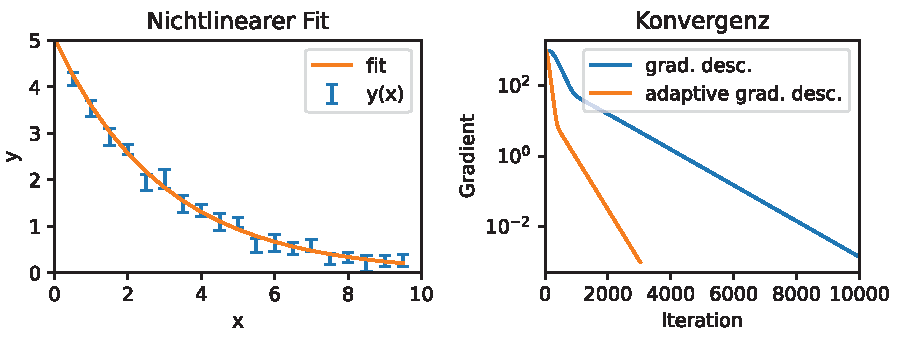
\includegraphics[width=0.8\textwidth]{Figures/nonlinear_fitting_image.pdf}
        \caption{Beispiel zum nichtlinearen Fitten. \textbf{Links:} Nichtlinearer Fit einer Exponentialfunktion zu fehlerbehafteten Daten. \textbf{Rechts:} Konvergenz des Gradientenverfahrens und des Newton-Verfahrens.  }
        \label{fig:nonlinearFit}
\end{figure} 

\subsection{Qualität des Fits}
\label{subsec:vl9-3}

Mit diesen Methoden können wir ausgehend von den Anfangswerten für die Fit parameter ein Minimum der Kostenfunktion $S$ bestimmen. Ob dieses Minimum jedoch das globale, oder ein lokales Minimum ist, ist nicht sicher. Wir könne das Ergebnis des Fits zusammen mit den Daten plotten um beurteilen zu können, ob die Daten gut beschrieben werden und ob nach unserer Vorstellung, das globale Minimum gefunden wurde.

Darüber hinaus, bietet es sich an die Residuen zu betrachten, um zu evaluieren, wie gut der Fit die Daten beschreibt (Siehe auch Abschnitt \ref{subsec:vl8-5-1}). Dazu berechnen wir $\epsilon_i =y_i - f(x_i, \boldsymbol{\hat{a}})$ für den gesamten Datensatz um die Modellparameter $\boldsymbol{\hat{a}}$ und $S$ zu minimieren. Idealerweise sollten die Abweichungen $\epsilon_i$ der gemessenen Werte $y_i$ von der Fitfunktion $f(x_i, \boldsymbol{\hat{a}})$ nur durch zufällige (statistische), unkorrelierte Fehler zustande kommen. In diesem Fall beschreibt unser Modell die Daten gut und die Voraussetzungen für die Berechnung der Unsicherheiten der Fitparameter (siehe \cref{eq:vl8-30}) sind erfüllt.\\
Wenn die Residuen nicht zufällig und symmetrisch um die Null verteilt sind, sondern systematische Abweichungen und Korrelationen aufweisen, dann beschreibt das Modell die Daten nur unzureichend (Wobei hier kleine Abweichungen oft nicht vermieden werden können und in Kauf genommen werden müssen). Diese Abweichung kann durch systematische Fehler in der Messung hervorgerufen werden, die durch eine Optimierung des Messaufbaus bzw. durch Anpassung des Modells reduziert oder vermieden werden können. Andererseits kann auch das physikalische Modell nicht das richtige sein, um den gemessenen Effekt zu beschreiben. Dann muss das Modell erweitert, oder ein anderes Modell gewählt werden. Es ist auf jeden Fall zu beachten, dass die Unsicherheiten der Fitparameter unzuverlässig sind wenn die Residuen zu starke Korrelationen aufweisen.



\subsection{Zusammenfassung}
\label{subsec:vl9-4}

\begin{itemize}
    \setlength\itemsep{0em}
        \item Wir können für jede Funktion die Kostenfunktion $S$ (die Summe der Abstandsquadrate) definieren.
        \item Minimieren von $S$ erlaubt uns die Funktionsparameter zu finden, für die die Funktion die Daten am besten beschreibt.
        \item Dazu folgen wir iterativ dem Gradienten von $S$ zum Minimum.
        \item Die Unsicherheit der Fitparameter können wir mit Hilfe der Hesse-Matrix berechnen.
        \item Die meisten Datenanalysewerkzeuge stellen effiziente und zuverlässige Implementationen dieser Methoden zu Verfügung, in Python z.B. ``curve\_fit'' in der ``scipy'' Bibliothek.
\end{itemize}


\newpage

\begin{tcolorbox}[enhanced,width=6in,
    fontupper=\small,drop fuzzy shadow southwest,
    colframe=black!50!black,colback=black!5]
\textbf{Verständnisfragen:} \\
\begin{enumerate}
\item[1] Was ist die Likelihood Funktion?
\item[2] Warum ist die Likelihood Funktion keine Wahrscheinlichkeitsverteilung? 
\item[3] Warum wollen wir die Likelihood Funktion maximieren? 
\item[4] Welchen Sinn hat die Log-Likelihood Funktion? 
\item[5] Was bedeuten die Residuen im Kontext eines Fit mit einer Ausgleichsgerade? 
\item[6] Was ist die Normalmatrix? 
\item[7] Warum funktioniert das invertieren der Normalmatrix nicht bei nichtlinearen Fitten? 
\item[8] Wie berechnet man die Unsicherheit der Fitparameter beim Nichtlinearen Fitten? 
\end{enumerate}
\end{tcolorbox}

\begin{tcolorbox}[enhanced,width=6in,
    fontupper=\small,drop fuzzy shadow southwest,
    colframe=black!50!black,colback=black!5]
\textbf{Antworten:} \\
\begin{enumerate}
\item[1] Die Likelihood Funktion gibt ein relatives Maß wie gut ein Modell mit Parametern $a_i$ zu bekannten Datenpunkten $x_i$ passt.
\item[2] Die Likelihood Funktion ist keine Wahrscheinlichkeiteverteilung, weil sie nicht normiert ist. 
\item[3] Die Parameter $a_i$, die die Likelihood Funktion maximieren, beschreiben die gemessenen Daten am besten, sodass wir ein aussagekräftigeres Modell erhalten. 
\item[4] Da die Likelihood Funktion nicht normiert ist, sind für uns nur relative Änderungen relevant. Oft erstrecken sich die Werte der Likelihood Funktion über viele Größenordnungen, sodass der Logarithmus der Likelihood Funktion ihre numerischen Werte besser vergleichbar macht. Zusätzlich können über die Log-Likelihood Funktion verschiedene Ausdrücke wie der Erwartungswert und die Varianz hergeleitet werden. 
\item[5] Die Residuen beim Fit mit einer Ausgleichsgerade sind die Abstände der Datenpunkte vom Fit Modell. Die gewichtete Summe der Residuen gibt an wie weit unsere Gerade von der optimalen Auslgeichsgerade entfernt ist.  
\item[6] Die Normalmatrix ist die Matrixform des linearen Gleichungssystems das man erhält wenn man die Summe der Residuen minimiert. Invertieren der Normalmatrix lässt uns aus den gemessenen Datenpunkten die Parameter eines Polynoms berechnen, das diese Datenpunkte optimal beschreibt. 
\item[7] Beim Ableiten der Summe der Residuen einer nichtlinearen Funktion ergibt sich nicht unbedingt ein lineares Gleichungssystem welches wir als Normalmatrix schreiben könnten. Daher müssen wir die Summe der Residuen iterativ minimieren.  
\item[8] Die Unsicherheiten der Parameter bei einem nichtlinearen Fit können abgeschätzt werden, indem man die nichtlineare Funktion entwickelt und dann behandelt wie eine lineare Funktion. 
\end{enumerate}
\end{tcolorbox}